\documentclass[11pt, letterpaper]{report}

%paquetes
\usepackage{tikz}
\usepackage{xcolor}
\usepackage{graphicx}
\usepackage{amsmath}
\usepackage{amssymb}
\usepackage[spanish, activeacute, es-noshorthands]{babel}
\usepackage{colortbl}
\usepackage{float}
\usepackage[utf8]{inputenc}
\usepackage[right = 2.5 cm, left = 2.5 cm, top = 2 cm , bottom = 2 cm]{geometry}
\usepackage{enumitem} %sirve para cambiar el tipo de enumeracion si redefinir comandos ejem: \arabic* \alph*

%configuraciones
\graphicspath{{img/}}
\newcommand{\Center}[1]{
	\begin{center}
		#1
	\end{center}
} %abreviatura para el ambiente center
\newcommand{\Page}[3][c]{
	\begin{minipage}[#1]{#2\textwidth}
		#3
	\end{minipage}
}
\renewcommand{\labelenumi}{$\bullet$} 
\newenvironment{enumTab}{\begin{enumerate}[label=]\item \begin{enumerate}[label=$\bullet$]}{\end{enumerate}\end{enumerate}} %comando para realizar enumeraciones con cierto margen
\newenvironment{block}[1]{\hspace{-0.8 cm}\textbf{\Large #1}}{\vspace{3 mm}} %ambiente importante que define una parte del reporte.
\newenvironment{question}[2]{\hspace{-0.8 cm}\textbf{#1) #2\\\\}}{\vspace{3 mm}} % define una pregunta, recibe como primer parametro al número y siguiente es la pregunta
\newcommand{\bib}[2]{ \textbf{\large #1:} \small #2\\} %forma sencilla de crear una referencia, como primer parametro recibe el titulo y el segundo el lugar a consultar
\newcommand{\note}[1]{\small \textbf{Nota:} #1} %comando que inserta una nota al texto
\spanishdecimal{.}
%comandos personales
%este commando sirve para crear bolas con enumeración
\newcommand*{\enumBall}[1]
		{
		\footnotesize\protect\tikz[baseline=-3pt]
		\protect\node[scale=.7, circle, ball color = white]{\color{black}\Large\bf #1};
		}
	
	
%%%%%%%%%%%%%%%%%%%%%%%%%%%%%%%%%%%%%%%%%%%%%%%%%%%%%%%%%%%%%%%%%%%%%%%%%%
%%%%%%%%%%%%%%%%%%%%%%% DOCUMENT BODY %%%%%%%%%%%%%%%%%%%%%%%%%%%%%%%%%%%%
%%%%%%%%%%%%%%%%%%%%%%%%%%%%%%%%%%%%%%%%%%%%%%%%%%%%%%%%%%%%%%%%%%%%%%%%%%	

\begin{document} 
	%%%%%%%%%%%%%%%%%%%%%%%%%%%%%%%%%%%%%
	%%%%%%%%%%%%% HEADER %%%%%%%%%%%%%%%%
	%%%%%%%%%%%%%%%%%%%%%%%%%%%%%%%%%%%%%
	%%%% BLOQUE DE DATOS %%%
\newcommand{\Title}{
	Práctica de Laboratorio \#3
	Multiplexores
} %Titulo del reporte

\newcommand{\LogoUniversity}{img/logo.jpg} %localizacion del logo
\newcommand{\NameUniversity}{Universidad Galileo} %Nombre de la universidad
\newcommand{\Date}{
	Guatemala, 6 de marzo de 2020
} %Fecha de entrega
\newcommand{\Faculty}{Facultad FISICC} %Nombre de la facultad
\newcommand{\Course}{
	Curso: Sistemas de Arquitectura
} %Nombre del curso
\newcommand{\ID}{
	Carnet: 1800 2955
}
\newcommand{\Student}{
	Alumno: Josu\'e Benyamin Isa\'i Galeano Morales
} %Nombre del estudiante
\newcommand{\Section}{
	Secci\'on: A
} %Sección del estudiante
\newcommand{\Schedule}{
	Horario de laboratorio: 18:00 a 19:00
} %Horario
\newcommand{\Assistant}{
	Auxiliar: Evelyn Cruz
} %Persona encargada
\newcommand{\Day}{
	Día de laboratorio: viernes
} %Dia en que recibe
%% FIN BLOQUE DE DATOS%%


%% NO ES NECESARIO MODIFICAR ESTA PARTE %%
\textbf{
	\small
	\hspace{-1 cm}
	\begin{minipage}{0.15\textwidth}
		%%%%%%%%%%%%%%%%% LOGO %%%%%%%%%%%%%%%%%%%%%%%%%%%%%%%
		\includegraphics[scale=0.5]{\LogoUniversity}
	\end{minipage}
	\begin{minipage}{0.7\textwidth}
		\resizebox{1.25\textwidth}{!}{
			\begin{tabular}{ll}
				\hline 
				%%%%% PARTE SUPERIOR DE LA TABLA DE DATOS %%%%%%%%%%%%%%%%%%%%%%%
				\NameUniversity & \Date \\
				\hline
				\rowcolor{lightgray}
				\Faculty & \Student\\
				\hline 
				\Course & \ID\\
				\hline\rowcolor{lightgray}
				\Section & \Schedule\\
				\hline 
				\Assistant & \Day\\
				\hline
			\end{tabular}
		}
	\end{minipage}
}

\vspace{0.5cm}
\begin{tikzpicture}
\hspace{-1 cm}
\draw (0.1,0.1) rectangle (1.043\textwidth,0.9);
\draw[line width=0.7mm] (0,0) rectangle (1.05\textwidth,1);
\node[font=\Large] at (0.525\textwidth, 0.45) {\textbf{\Title}};
\end{tikzpicture}		

\vspace*{0.5 cm}
 %incluimos la parte del header en el documento, note que header es como escribir dentro de un ambiente document por lo tanto no debe llevar definición de clase ni definiciones que se hagan exclusivamente en el preambulo.
	
	%%%%%%%%%%%%%%%%%%%%%%%%%%%%%%%%%%%%%
	%%%%%%%%%%%% OBJETIVOS %%%%%%%%%%%%%%
	%%%%%%%%%%%%%%%%%%%%%%%%%%%%%%%%%%%%%
	\begin{block}{Objetivos:}
		\begin{enumTab}
			\item Comprender para que sirve el punto de operaci\'on y como se afecta cuando esta en polarizaci\'on por divisor de voltaje.
		\end{enumTab}
	\end{block}
	
	%%%%%%%%%%%%%%%%%%%%%%%%%%%%%%%%%%%%%
	%%%%%%%%%%%%% RESUMEN %%%%%%%%%%%%%%%   
	%%%%%%%%%%%%%%%%%%%%%%%%%%%%%%%%%%%%%		
	\begin{block}{Resumen:}
		
		En la pr\'actica se busc\'o informaci\'on sobre el BJT, con la cual se armaron los circuitos prove\'idos en el archivo del laboratorio, despu\'es de haberlo terminado de armar, se procedi\'o a calcular el $V_B$, $I_E$ y $V_{CE}$.
	\end{block}
		
	%%%%%%%%%%%%%%%%%%%%%%%%%%%%%%%%%%%%%
	%%%%%%%%%%%%% TEORIA %%%%%%%%%%%%%%%%
	%%%%%%%%%%%%%%%%%%%%%%%%%%%%%%%%%%%%%
	\begin{block}{Teor'ia:}
	
		\textbf{BJT} Es un componente semiconductor el cual se modela como una fuente de corriente controlada por corriente, esto es debido que la corriente del colector es directamente proporcional a la corriente en la base,.
		
		
		\begin{figure}[H]
			\Center{
				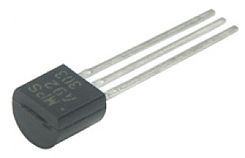
\includegraphics[scale=.4]{BJT.jpg}
				\caption{\textbf{BJT}}
			}
		\end{figure}
	
		\textbf{Punto de operaci\'on} Es la coordenada denotada por ($V_{CE}$,$I_C$) en el plano cartesiano $R^2$ donde el eje de las abscisas es nombrado por el voltaje de colector a emisor y el de las ordenadas por la corriente en el colector, este punto es fijo y representa como su nombre lo dice el punto donde est\'a operando.
		
		\textbf{Recta de Carga} cuando el punto de operaci\'on se ve afectada por causa de cambios en Vcc, etc, el nuevo punto quedará sobre dicha recta.
		
	
	\end{block}
		
	%%%%%%%%%%%%%%%%%%%%%%%%%%%%%%%%%%%%%
	%%%%%%%%%% DATOS PRACTICOS %%%%%%%%%%
	%%%%%%%%%%%%%%%%%%%%%%%%%%%%%%%%%%%%%
	\begin{block}{Datos Pr'acticos:}
		
		\vspace*{.5cm}
		\Page{.5}{
			\begin{figure}[H]
				\Center{
					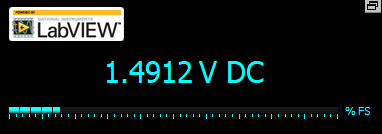
\includegraphics[scale=.5]{Vce.png}
					\caption{\textbf{Voltaje Colector Emisor}}
				}
			\end{figure}
		}
		\Page{.5}{
			\begin{figure}[H]
				\Center{
					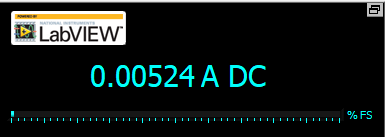
\includegraphics[scale=.5]{Ie.png}
					\caption{\textbf{corriente Emisor}}
				}
			\end{figure}
		}
	
		\begin{figure}[H]
			\Center{
				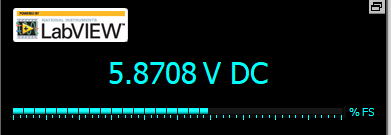
\includegraphics[scale=.4]{Vb.PNG}
				\caption{\textbf{Voltaje Base}}
			}
		\end{figure}
	
	\end{block}
	
	%%%%%%%%%%%%%%%%%%%%%%%%%%%%%%%%%%%%%
	%%%%%%%%% CALCULOS TEORICOS %%%%%%%%%
	%%%%%%%%%%%%%%%%%%%%%%%%%%%%%%%%%%%%%
	\begin{block}{C\'alculos Te\'oricos:\\}
		
		\textbf{an\'alisis aproximado}\\
		\Page{.33}{$100\leq\beta\leq300\therefore 10R_2 \leq\beta R_E$}
		\Page{.2}{$V_B=12\frac{1k\Omega}{2k\Omega}=6V$}
		\Page{.2}{$I_E=\frac{5.3V}{1k\Omega}=5.3mA$}
		
		\hspace*{-.5cm}$V_{CE}=12V-I_CR_C-I_ER_E=1.4V$
		
	\end{block}
			
	%%%%%%%%%%%%%%%%%%%%%%%%%%%%%%%%%%%%%
	%%%%%%%%%%% CONCLUSIONES %%%%%%%%%%%%
	%%%%%%%%%%%%%%%%%%%%%%%%%%%%%%%%%%%%%
	\vspace{3 mm}
	\begin{block}{Conclusiones:}
	\begin{enumTab}
		\item El an\'alisis de un circuito polarizado por divisor de voltaje puede volverse muy sencillo si se cumple la regla $10R_2 \leq\beta R_E$.
		\item Conocer la recta de carga es importante para saber la posici\'on de cualquier punto operaci\'on del BJT.
	\end{enumTab}
	\end{block}
		
		
	%%%%%%%%%%%%%%%%%%%%%%%%%%%%%%%%%%%%%
	%%%%%%%%%%% BIBLIOGRAFIA %%%%%%%%%%%%
	%%%%%%%%%%%%%%%%%%%%%%%%%%%%%%%%%%%%%
	\begin{block}{Bibliograf'ia:}
	
		\bib{BJT - Wikipedia}{https://es.wikipedia.org/wiki/Transistor\_de\_uni\%C3\%B3n\_bipolar}
	\end{block}
		
\end{document}
